In Figure \ref{fig: slices_StokesI} we present plots of the \stokesI values along the slices along the minor axis for all 4 bands. When we look at the slices in \SIns, we can see that the shapes are all centred at the origin.

% \begin{figure*}[h]
%   \centering
%   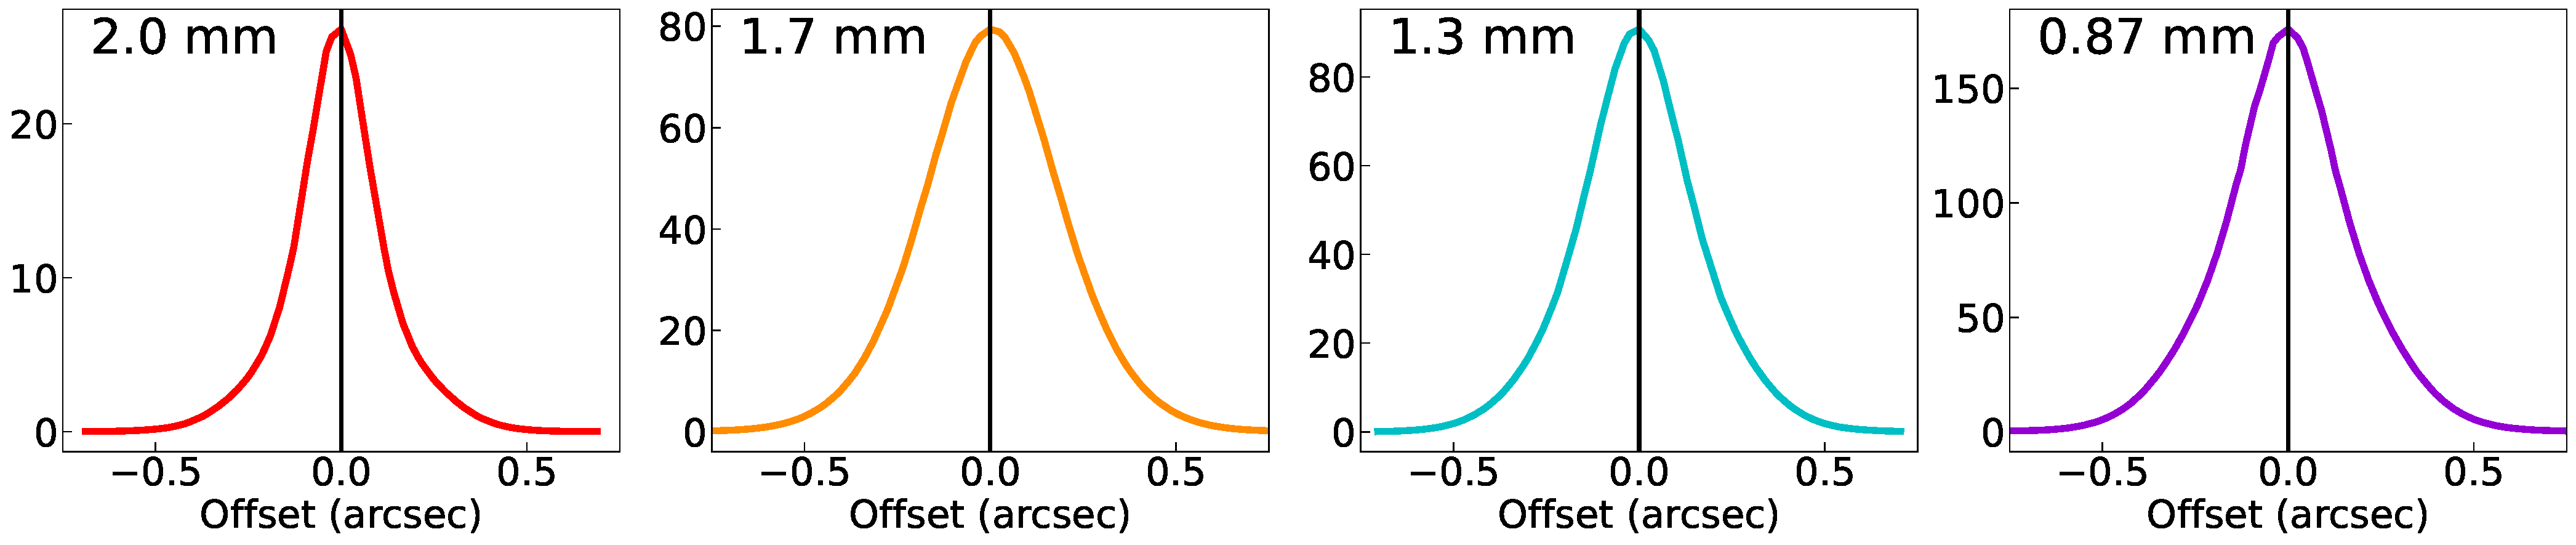
\includegraphics[width=1.1\textwidth]{WRITEUP_AND_IMAGES/IMAGES/WRITEUP/Slices/MW_slices_StokesI.pdf}
%   \caption{Plot of Stokes I in mJy versus offset from the centre position of the disk. The centre position values can be found in Figure \ref{tab: source_info}, and the slices are shown in Figure \ref{fig: slice-along-minor}. A solid black line is shown at a offset of 0. }
%   \label{fig: slices_StokesI}
% \end{figure*}


\begin{figure*}[h]
  \centering
  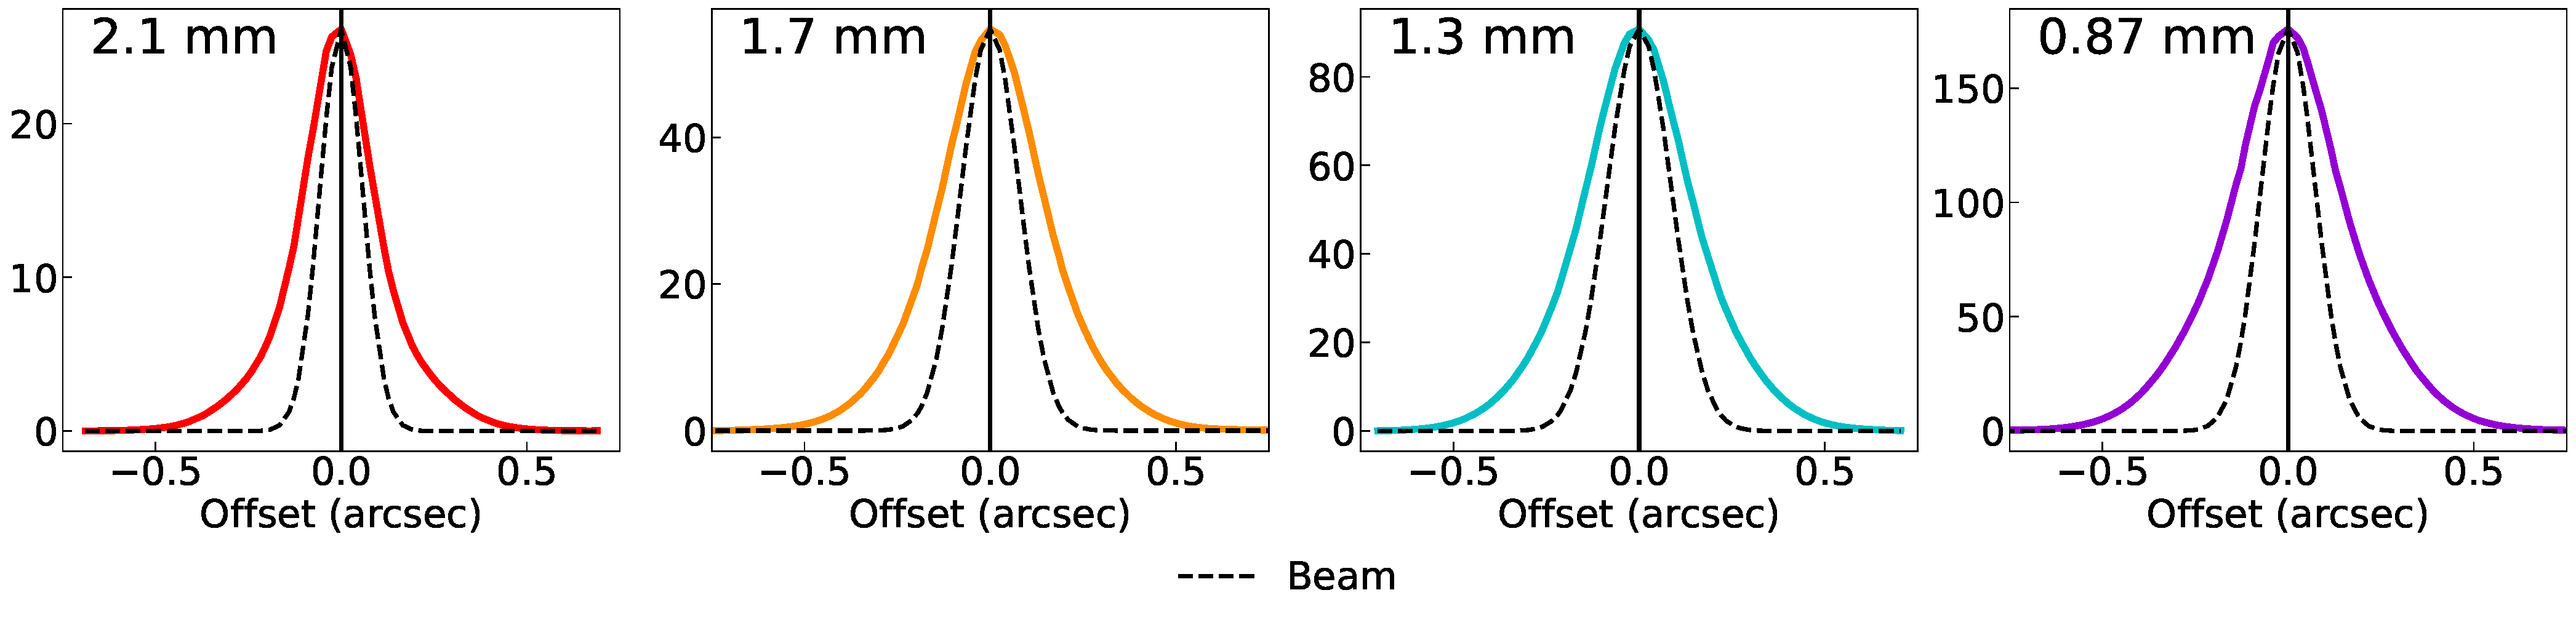
\includegraphics[width=1.1\textwidth]{WRITEUP_AND_IMAGES/IMAGES/WRITEUP/Slices/MW_slices_StokesI_with_beam.pdf}
  \caption{Plot of Stokes I in mJy versus offset from the centre position of the disk. The centre position values can be found in Figure \ref{tab: source_info}, and the slices are shown in Figure \ref{fig: slice-along-minor}. A solid black line is shown at a offset of 0. }
  \label{fig: slices_StokesI}
\end{figure*}



This tells us that when we look at all of the light from the disk (polarized or not), we see the most light at the centre of the disk. This is expected, as the young star is at the centre of the disk, so it should be brightest there.